\documentclass[aspectratio=169,11pt]{beamer}
\usetheme{default}
\usecolortheme{seahorse}
\setbeamertemplate{navigation symbols}{}
\setbeamertemplate{footline}[frame number]
\usepackage[utf8]{inputenc}
\usepackage[T1]{fontenc}
\usepackage{booktabs,graphicx,amsmath}
\title{Can Opponent Learning Compensate for Limited Communication?}
\subtitle{Multi-agent reinforcement learning for cooperative pursuit}
\author{Piyush Choudhary (23110247) \and Shivansh Shukla (23110303)}
\date{}
\begin{document}

\begin{frame}
\titlepage
\end{frame}

\begin{frame}{1. The problem}
\begin{columns}[T]
\column{0.58\textwidth}
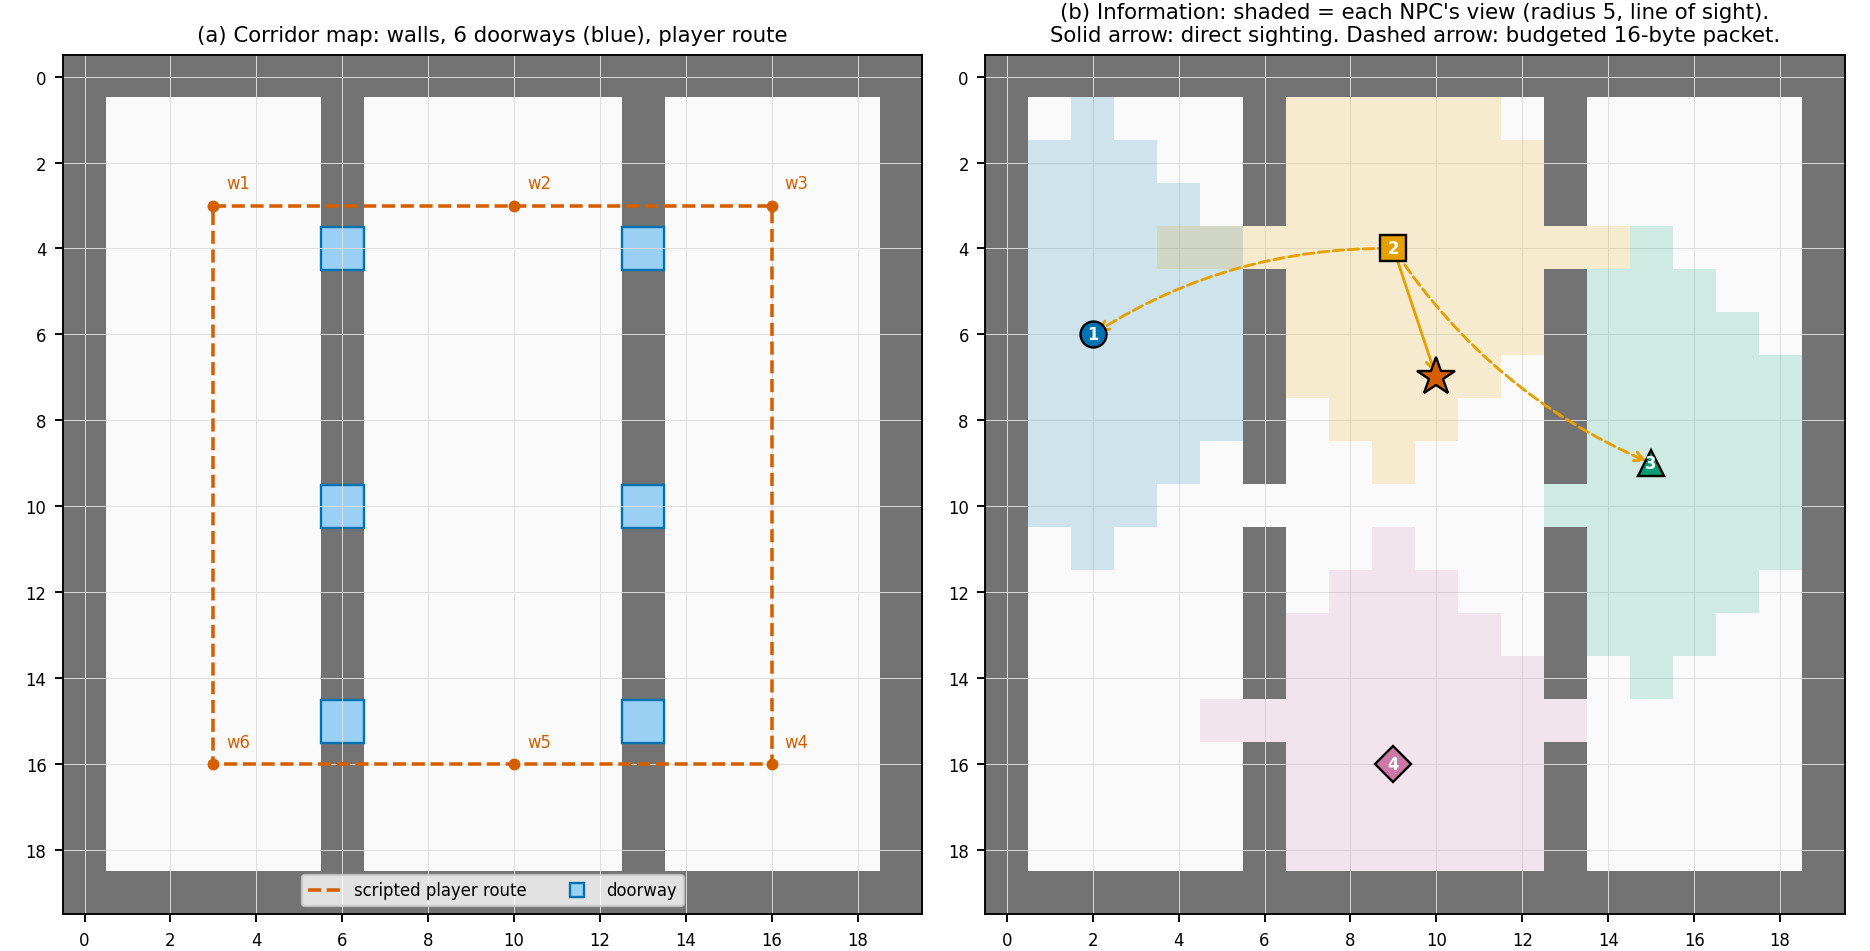
\includegraphics[width=\linewidth]{figures/map_information.png}
\column{0.4\textwidth}
\begin{itemize}
\item Four NPCs chase one player in a corridor map.
\item Each NPC sees only radius 5, with line of sight.
\item One NPC may see the player; the others see empty space.
\end{itemize}
\textbf{Question:} can a learned model of the player make up for scarce messages?
\end{columns}
\end{frame}

\begin{frame}{2. What each NPC knows}
\begin{itemize}
\item Knows: the map, its own position and ID, time, budget $B$.
\item Sees: visible cells and the agents in them.
\item Hears: 16-byte broadcast packets from teammates, delivered at the next step.
\item Budget rule: send only if $\mathrm{sent}_i<\lfloor B(t+1)\rfloor$, for $B\in\{0,\tfrac18,\tfrac12,1\}$.
\item Never available: the player's hidden position, its route phase, or other NPCs' private state.
\end{itemize}
\end{frame}

\begin{frame}{3. Four methods}
\begin{tabular}{p{2.2cm}p{9cm}}
\toprule
\textbf{IP} & Shortest path to the last direct sighting; otherwise search. Sends nothing.\\
\textbf{RC} & Shared role hints (chase, intercept, block, search); sends on sightings and role changes.\\
\textbf{MARL} & Recurrent MAPPO: GRU actor, centralized critic, joint move-and-send action.\\
\textbf{MARL-OM} & MARL plus a local predictor of the player's next move and a belief over its position.\\
\bottomrule
\end{tabular}
\vspace{4pt}

Three learners are kept separate: the pursuers' policy, the opponent model, and the player's own learning.
\end{frame}

\begin{frame}{4. Scripted and learning players}
\begin{itemize}
\item \textbf{Waypoint player:} fixed route, random move with probability $\xi\in\{0,0.25,0.75\}$.
\item \textbf{Q-learning player:} updates a tabular policy after every step ($\epsilon=0.10$).
\item Eight Q checkpoints: three for validation, five held out.
\item The learning player is used in frozen and adapting modes to test transfer and tracking.
\end{itemize}
\end{frame}

\begin{frame}{5. Pilot evidence and training budget}
\begin{itemize}
\item Pilots at 300k, 600k and 1.2M transitions; 1.2M chosen as the common budget.
\item All six required waypoint conditions reach capture $\ge 0.20$ and improve by $\ge 0.10$ over the untrained policy.
\item Task calibration: message use audited; four task variants compared on validation seeds; original task retained.
\end{itemize}

\end{frame}

\begin{frame}{6. Capture versus communication}
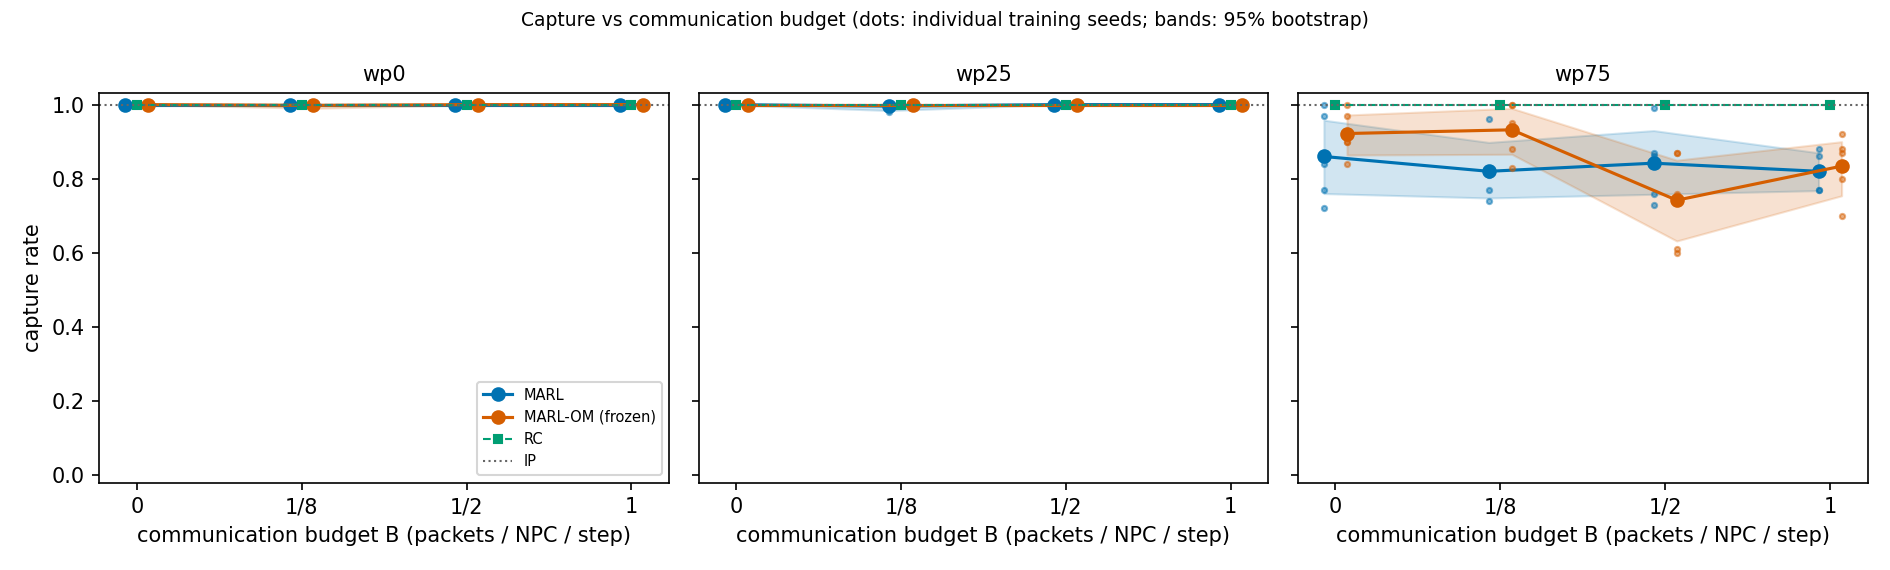
\includegraphics[width=\linewidth]{figures/capture_vs_budget_waypoint.png}
\begin{itemize}
\item $\xi\le0.25$: every method at ceiling (capture $\ge0.996$).
\item $\xi=0.75$, $B=1/8$: MARL-OM 0.93 vs MARL 0.82, $G=+0.11$ (95\% CI $-0.01$ to $0.22$); Holm $p=0.56$.
\end{itemize}
\end{frame}

\begin{frame}{7. Actual communication}
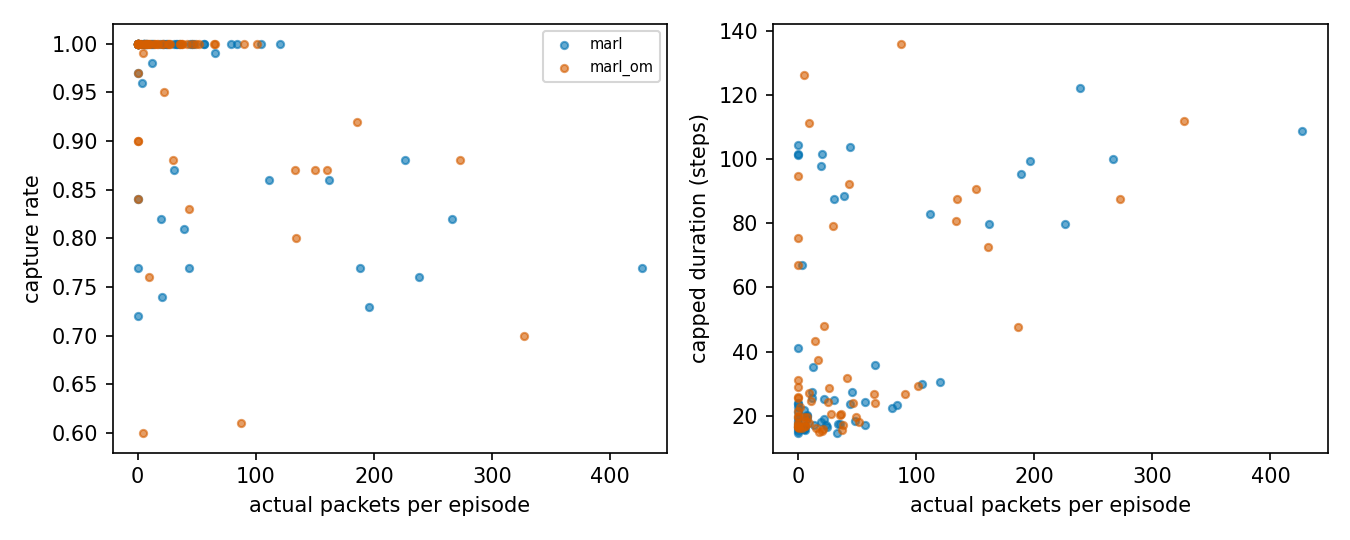
\includegraphics[width=0.9\linewidth]{figures/packets_vs_capture.png}

Most runs send few packets (under about 100 per episode) and capture almost every episode; the runs that send many packets are the ones with lower capture and longer episodes.
\end{frame}

\begin{frame}{8. Adaptive player}
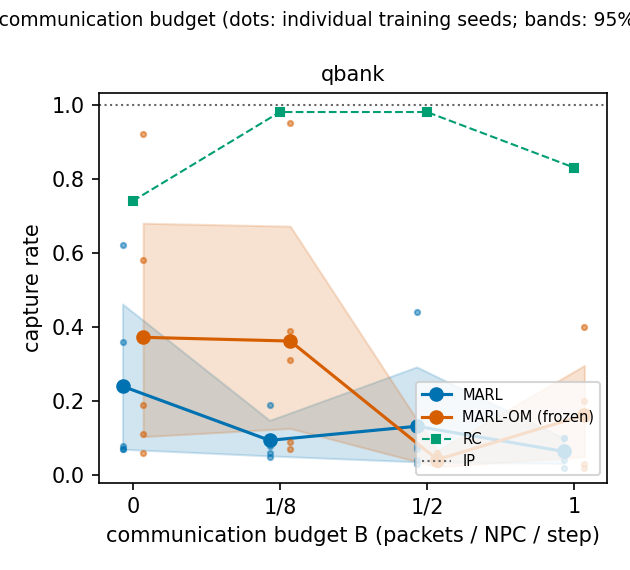
\includegraphics[width=0.55\linewidth]{figures/capture_vs_budget_player.png}
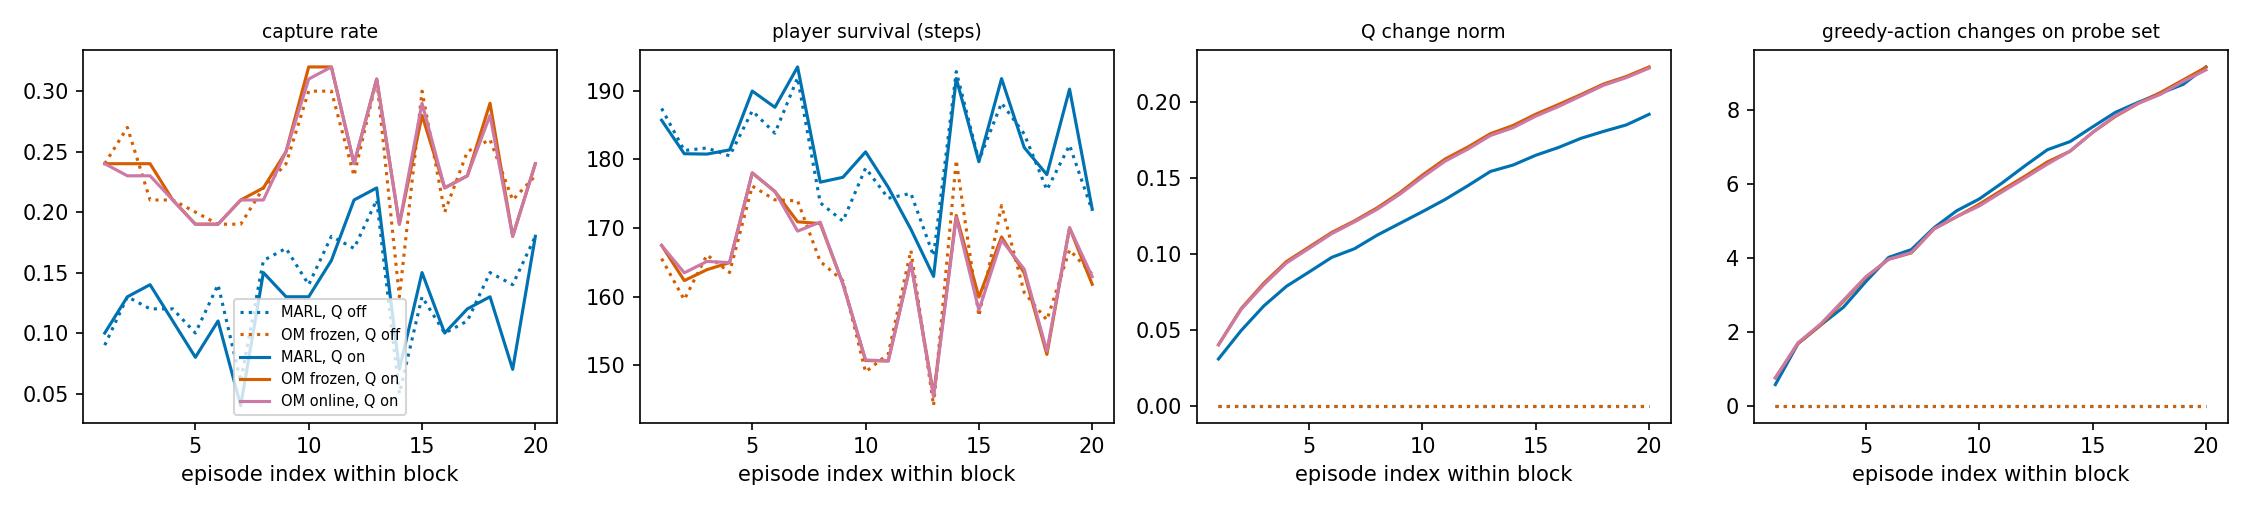
\includegraphics[width=0.4\linewidth]{figures/adaptive_curves.png}
\begin{itemize}
\item Transfer to held-out Q players, $B=1/8$: MARL-OM 0.36 vs MARL 0.09, $G=+0.27$ (CI $0.01$ to $0.58$); Holm $p=0.19$.
\item Online vs frozen predictor within 20-episode blocks: differences $\le0.002$ (exploratory).
\end{itemize}
\end{frame}

\begin{frame}{9. Short replay}
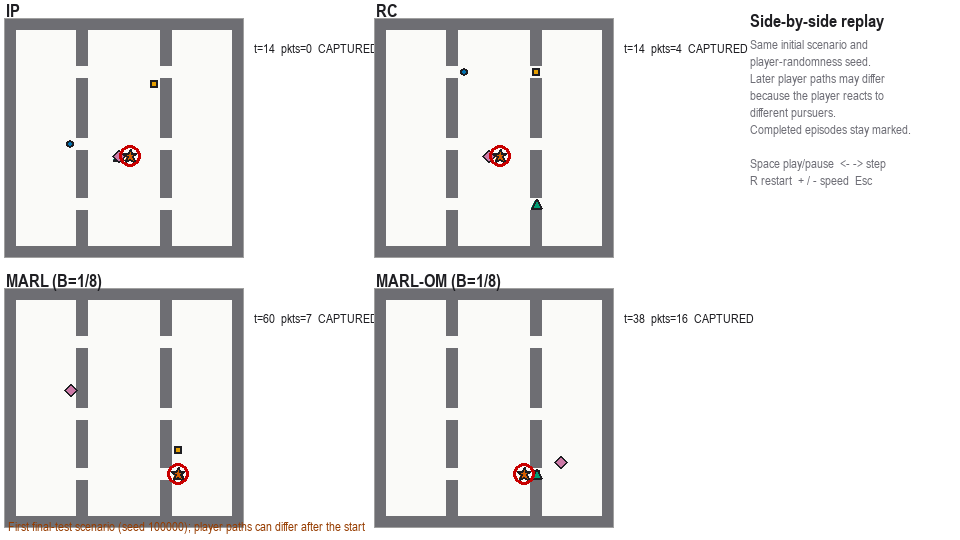
\includegraphics[width=0.32\linewidth]{figures/keyframe_06_scene2_t060.png}
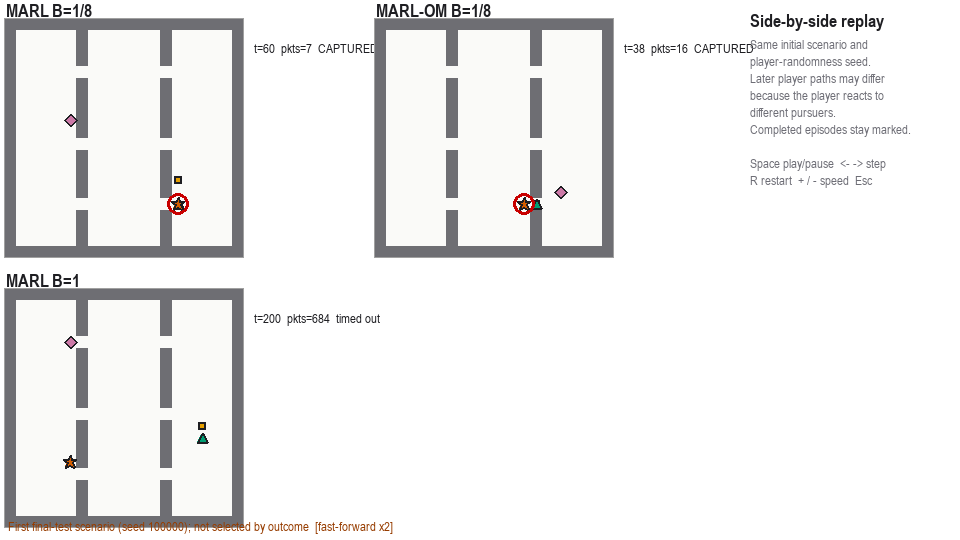
\includegraphics[width=0.32\linewidth]{figures/keyframe_09_scene3_t200.png}
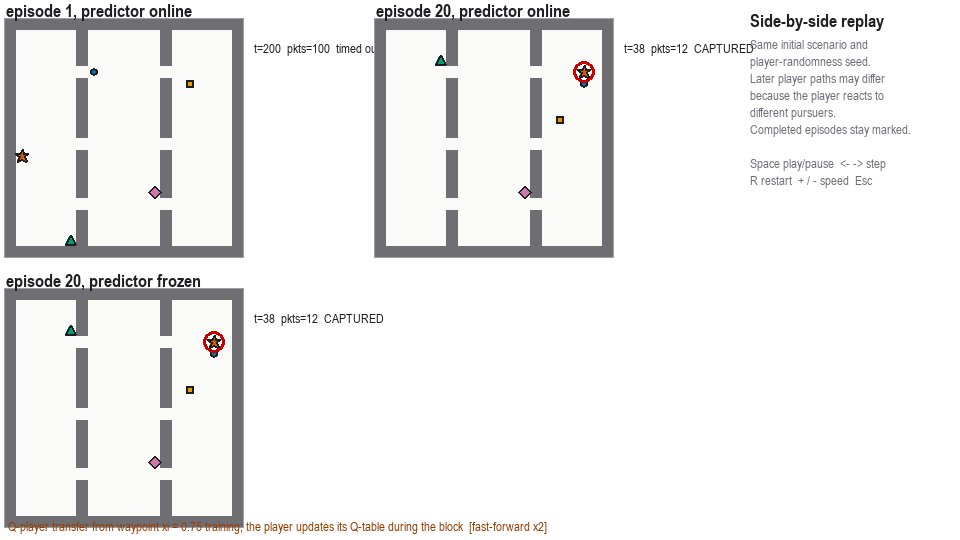
\includegraphics[width=0.32\linewidth]{figures/keyframe_12_scene4_t200.png}

Recorded comparison scenes (methods, budgets, learning player); the full 90 s \texttt{demo.gif} is in the evaluator pack.
\end{frame}

\begin{frame}{10. Conclusions and contributions}
\begin{itemize}
\item At ceiling for $\xi\le0.25$; headroom only at $\xi=0.75$ and on the Q player.
\item MARL-OM has higher point estimates at low budget; five-seed tests do not confirm them.
\item Online predictor updates: no measurable effect in these blocks.
\item 120 paired runs, bootstrap intervals, every run kept.
\end{itemize}

\textbf{Piyush:} simulator, players, IP/RC, tests, rendering and viewer.\quad
\textbf{Shivansh:} MAPPO, predictors, protocols, statistics, plots.\quad
\textbf{Both:} protocol, experiments, report, slides, demo.
\end{frame}

\appendix
\begin{frame}{Backup: formulation}
$r=\mathbf 1[\text{capture}]-\tfrac{0.10}{H}-\tfrac{0.01\,b_t}{NH}-\tfrac{0.02\,m_t}{NH}$, $\gamma=1$, $H=200$.\\[4pt]
Packet: 16 bytes (sender, flags, sender cell, target cell, target step, displacement, role, destination, send step, padding).
\end{frame}

\end{document}
